\documentclass{beamer}


\begin{document}
% 1. Front slide
\begin{frame}
\frametitle{Zero-inflated models}
Mark Greenaway
% Details about myself here?
\end{frame}

% 2. Intro
\begin{frame}
\frametitle{Introduction}
Zero inflated data arises in many areas of application, such as physical
activity data, number of hospital visits and number of insurance claims per
year.

We will work with zero-inflated count data.
\end{frame}

% 3. Univariate model
\begin{frame}
\frametitle{Univariate model formulation}
We start by building a relatively simple zero-inflated count model.
\begin{align*}
X_i &= R_i Y_i \\
R_i &\sim \text{Bernoulli}(\rho) \\
Y_i &\sim \text{Poisson}(\lambda) \\
\rho &\sim \text{Beta}(a_\rho, b_\rho) \\
\lambda &\sim \text{Gamma}(a_\lambda, b_\lambda) \\
\end{align*}
\end{frame}

% 4. \rho = 9/10, \lambda = 5
% Example data 0 0 0 5 10
\begin{frame}
\frametitle{Example data}
Take, for example, $\rho = \frac{1}{2}$, $\lambda = 5$.
\begin{verbatim}
0 7 3 4 5 3 2 6 5 0 0 1
0 0 5 0 2 3 6 4 0 5 4 0
7 0 0 0 7 0 6 6 0 3 0 5
0 4 0 0 0 2 3 0 3 4 5 0
8 0
\end{verbatim}
% Histogram
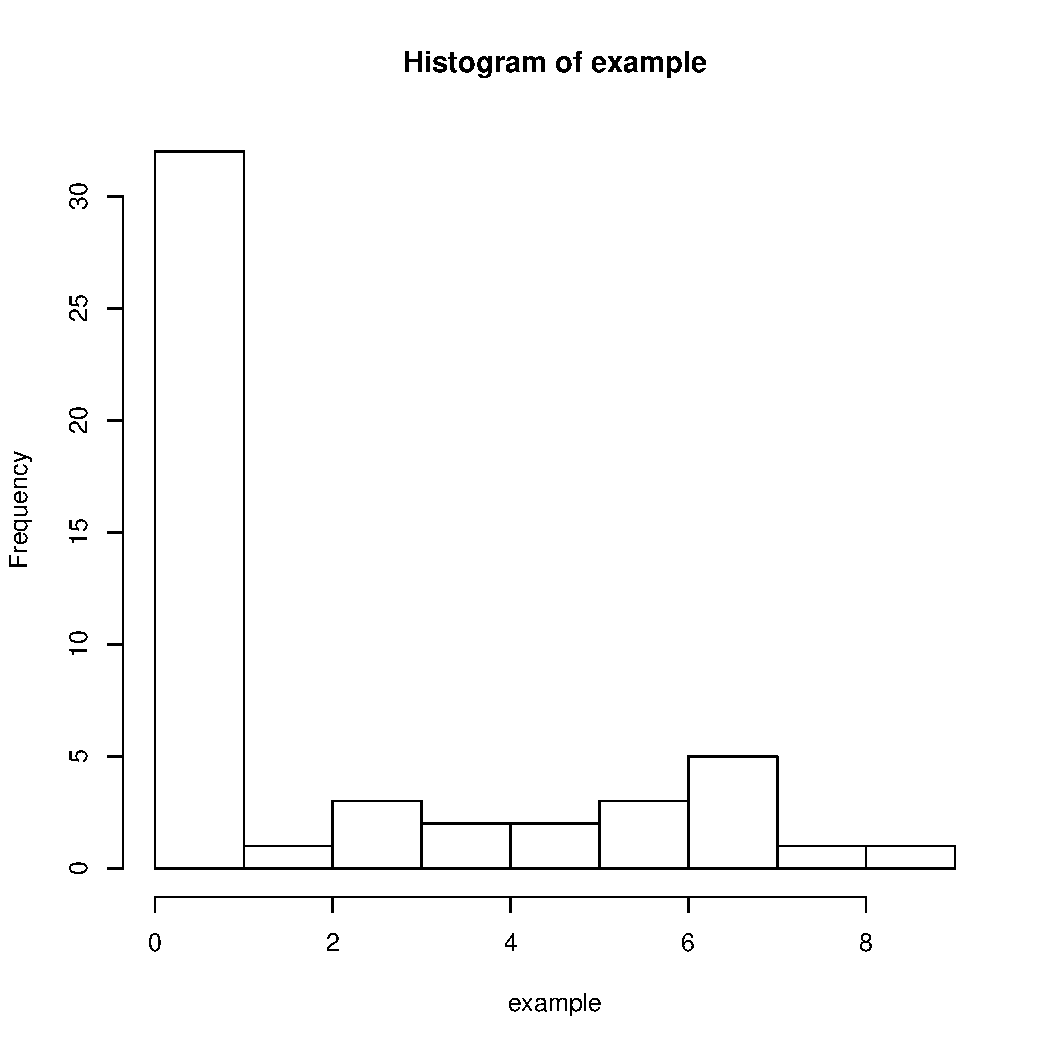
\includegraphics{code/univariate_data_histogram.pdf}
% Density
\end{frame}

% 5. How to fit, and advantages and disadvantages of each approach
% - Maximum likelihood
% - MCMC
% - VB
\begin{frame}
\frametitle{Comparison of techniques}
Maximum likelihood
Frequentist
\begin{array}{ll}
Pro & Con \\
Standard optimisation techniques can be used & Biased for mixed models 
\end{array}

MCMC
\begin{array}
Pro & Con \\
Very accurate & Slow \\
& May not converge at all
\end{array}

Variational Bayes
\begin{array}{ll}
Pro & Con \\
Fast & May lose accuracy, variance \\
Still quite accurate & Solution may be intractable
\end{array}

\end{frame}

% 6. Overview of Variational Bayes
\begin{frame}
\frametitle{An overview of Variational Bayes}
\begin{itemize}
\item Approximate the full posterior p(\theta) with an approximation q(\theta)
\item Minimise the KL divergence between p(\theta) and q(\theta)
\item Theory guarantees that p(\theta) < q(\theta) and that q(\theta) will
increase with each VB step
\end{itemize}
\end{frame}

% 7a. Variational Bayes solution to ZIP
% - q-densities
\begin{frame}
Choose a factored approximation of the form
$$
q(\theta) = q(\lambda) q(\rho) \prod_{i=1}^n q(r_i)
$$
where
$$
q(\lambda) = \text{Gamma}(a_\lambda_*, b_\lambda_*)
q(\rho) = \text{Beta}(a_{q(\rho)}, b_{q(\rho))
q(r_i) = Bernoulli(p_i)
$$

% - Algorithm
We iteratively update the parameters of each approximate distribution
in turn until the lower bound of the approximation converges.

This could be thought of as a generalisation of Expectation Maximisation,
where each parameter is thought of as the unobserved parameter and maximised
relative to the other parameters in turn..
% FIXME - Check this.
\end{frame}

% 8. Results
% - Lower bound convergence
% - Accuracies
% 7b. Define accuracy
\begin{frame}
\frametitle{Mean field updates}
% Are they going to be happy with that?
Most of the mean field updates are straightforward, as the priors are conjugate.
$$
q(\lambda) = \text{Gamma}(\alpha_\lambda + \vone^T \vx, \beta_\lambda + \vone^T\vp)
q(\rho) = \text{Beta}(\alpha_\rho + \vone^T\vr, \beta_\rho + \vone^T(\vone - \vr))
$$
$$
q(r_i) = \text{Bernoulli}(\text{expit}(\eta_i))
$$
where
$$
\eta_i = - \frac{\alpha_\lambda^*}{\beta_\lambda^*} + \Psi(\alpha_\rho^*) - \Psi(\beta_\rho^*)
$$
\end{frame}

\begin{frame}
\frametitle{Results/Accuracy}
% Definition of accuracy
Accuracy is defined as the difference in $L_1$ norm between the true posterior distribution and
the approximate posterior distribution of the variational approximation. This was calculated
using the kernel density estimate of the posterior distribution from MCMC minus the approximate
distribution for each parameter of interest.

Excellent accuracy for the univariate approximation, over 99\% in all of the cases that I looked at.
% Graph of lower bound
%\includegraphics{univariate_lower_bound_convergence.pdf}
\end{frame}

% 9. Extension to linear model
% 10. Overview GVA
% 11. Algorithm
% 12. Results?
% 13. What next
% 14. Conclusion
% 15. References
\begin{frame}
\frametitle{Extension to multivariate/regression models}
Extension from univariate, model formulation
$$
q(\theta) = q(\beta) q(\rho) \prod_{i=1}^n q(r_i)
$$
where
$q(\beta) \sim N(\mu, \Sigma)$ and
$q(\sigma_u^2) \sim IG(\alpha_{\sigma_u^2}, \beta_{\sigma_u^2})$

\begin{itemize}
\item Mixed models -- one model to rule them all
\item The need for better approaches - MCMC with existing software can take minutes to
converge, if they converge at all. That might not sound so bad to you, but how do you
do model selection?
\end{itemize}
\end{frame}

\begin{frame}
\begin{itemize}
\item Lack of conjugacy means mean field updates won't be analytically tractable.
\item We try Gaussian Variational Approximations instead, assume that $\beta, \vu \sim N(\vmu, \Sigma)$
and approximate as closely as we can
\item Computation - a work in progress
\item Initial signs are that this approach will work. Parameters are correctly estimated for simulated data.
\end{itemize}
\end{frame}

\begin{frame}
\frametitle{Further work}
\begin{itemize}
\item Continue working on the multivariate approximation
\item Check accuracy against random walk Metropolis-Hastings
\end{itemize}
\end{frame}

\begin{frame}
\frametitle{References}
\begin{itemize}
\item Explaining variational approximations
\item Gaussian variational approximations
\item General Design Mixed Models
\end{itemize}
\end{frame}

\end{document}
